\section{Study 1: what a learned projection removes, and what it breaks}
\label{sec:study1}

\subsection{How much the agent uses, and how much a projection removes}

Table~\ref{tab:phasea} summarises Phase A. Only a minority of the tool-output tokens carry fields the agent
visibly used (with the record keys): \PhaseAUsedSharei{} in the editorial plan, \PhaseAUsedShareiii{} in the
literature scan, \PhaseAUsedShareiv{} and \PhaseAUsedSharev{} in the two simulated cases. On runs it had not seen,
the prudent projection removed \PhaseAPrudentSavingi, \PhaseAPrudentSavingiii, \PhaseAPrudentSavingiv{} and
\PhaseAPrudentSavingv{} of the tool-output tokens of these cases; in the editorial plan this is above the 30\%
threshold of H1, which holds. Part of each figure involves no removal at all: the tools return indented JSON, and
writing the same payload compactly and without escapes already removes \ReserialAi{} in the editorial plan,
\ReserialAiv{} in billing support and \ReserialAv{} in CI triage (column \emph{Re-serialised}), and almost nothing
in the literature scan, whose outputs were already compact. The content-gap analyst is the boundary case: it cites
most of what search results contain (URLs, titles, snippets) and its page parses are prose, which a field projection
cannot touch; its projection removed \PhaseAPrudentSavingii. Without the \PhaseASensExcludedi{} editorial-plan
runs in which a tool call failed (deviation 6), the saving there is \PhaseASensSavingi{} and the misses
\PhaseASensMissesi.

\begin{table}[t]
\centering\small
\resizebox{\textwidth}{!}{\begin{tabular}{lrrrrrrrrr}
\toprule
Case & Runs & Calls & Tool-output tokens & Used & Re-serialised & Prudent & Aggressive & Misses & Misses (calls only) \\
\midrule
Editorial plan & 8 & 173 & 817{,}865 & 32\% & $-$13\% & $-$63\% & $-$68\% & 2/166 & 69/166 \\
Content gaps & 8 & 136 & 527{,}542 & 84\% & $-$4\% & $-$12\% & $-$16\% & 9/90 & 26/90 \\
Literature scan & 8 & 61 & 2{,}262{,}885 & 19\% & 0\% & $-$70\% & $-$81\% & 3/61 & 61/61 \\
Billing support$^\dagger$ & 8 & 84 & 154{,}833 & 17\% & $-$17\% & $-$69\% & $-$84\% & 9/84 & 61/84 \\
CI triage$^\dagger$ & 8 & 104 & 599{,}808 & 18\% & $-$7\% & $-$77\% & $-$82\% & 3/64 & 64/64 \\
\bottomrule
\end{tabular}
}
\caption{Phase A, eight live runs per case. \emph{Used}: share of tool-output tokens left by the in-sample
aggressive projection (used fields and record keys), a lower bound of use. \emph{Re-serialised}: change from
re-serialising each JSON output compactly, with no field removed (the lossless part of the next two columns).
\emph{Prudent}, \emph{Aggressive}:
change in tool-output tokens on held-out runs. \emph{Misses}: held-out calls in which the aggressive projection
removes a field the run used later, learning from everything the agent wrote, or only from tool calls.
$^\dagger$Simulated tools.}
\label{tab:phasea}
\end{table}

\begin{figure}[t]
\centering
% Generated by experiments/paper_figures.py. Do not edit.
\definecolor{ttgray}{HTML}{9A9893}\definecolor{ttblue}{HTML}{2A78D6}\definecolor{ttorange}{HTML}{EB6834}\definecolor{ttaqua}{HTML}{1BAF7A}\definecolor{ttgrid}{HTML}{DDDCD8}\definecolor{ttmuted}{HTML}{52514E}
\begin{tikzpicture}
\begin{axis}[axis x line*=bottom, axis y line*=left, axis line style={draw=ttmuted}, tick style={draw=none}, major grid style={draw=ttgrid}, tick label style={font=\footnotesize}, label style={font=\footnotesize}, legend style={font=\footnotesize, draw=none, fill=none}, legend cell align=left, name=C4, width=0.78\linewidth, height=4.10cm, xbar stacked, bar width=7pt, xmin=0, xmajorgrids, xlabel={thousand tokens, held-out runs}, ytick={0,...,4}, yticklabels={{\texttt{\scriptsize stripe\_list\_invoices}},{\texttt{\scriptsize stripe\_list\_charges}},{\texttt{\scriptsize stripe\_search\_customers}},{\texttt{\scriptsize stripe\_list\_subscriptions}},{\texttt{\scriptsize stripe\_list\_refunds}}}, y dir=reverse, enlarge y limits=0.12, title={\footnotesize Billing support: 57\% removed}, legend to name=toolslegend, legend columns=2, area legend, ]
\addplot[fill=ttblue, draw=white, line width=0.6pt] coordinates {(30.1,0) (19.2,1) (13.7,2) (3.8,3) (0.2,4)};
\addlegendentry{kept}
\addplot[fill=ttorange, draw=white, line width=0.6pt] coordinates {(44.5,0) (21.3,1) (16.2,2) (5.3,3) (0.5,4)};
\addlegendentry{removed}
\end{axis}
\begin{axis}[axis x line*=bottom, axis y line*=left, axis line style={draw=ttmuted}, tick style={draw=none}, major grid style={draw=ttgrid}, tick label style={font=\footnotesize}, label style={font=\footnotesize}, legend style={font=\footnotesize, draw=none, fill=none}, legend cell align=left, name=C5, width=0.78\linewidth, height=4.10cm, xbar stacked, bar width=7pt, xmin=0, xmajorgrids, xlabel={thousand tokens, held-out runs}, ytick={0,...,4}, yticklabels={{\texttt{\scriptsize gh\_list\_pull\_requests}},{\texttt{\scriptsize gh\_list\_issues}},{\texttt{\scriptsize gh\_list\_workflow\_runs}},{\texttt{\scriptsize gh\_download\_job\_logs}},{\texttt{\scriptsize gh\_list\_jobs\_for\_workflow\_run}}}, y dir=reverse, enlarge y limits=0.12, title={\footnotesize CI triage: 61\% removed}, at={(C4.south west)}, anchor=north west, yshift=-2.1cm, ]
\addplot[fill=ttblue, draw=white, line width=0.6pt] coordinates {(47.4,0) (51.5,1) (22.3,2) (92.8,3) (18.4,4)};
\addplot[fill=ttorange, draw=white, line width=0.6pt] coordinates {(130.7,0) (90.0,1) (92.1,2) (0.0,3) (54.6,4)};
\end{axis}
\node[anchor=north] at ($(C5.south)+(0,-0.95)$) {\pgfplotslegendfromname{toolslegend}};
\end{tikzpicture}

\caption{Where the tokens go, per tool, in the two cases with simulated tools (released in full): tool-output
tokens on held-out runs, split into what the prudent projection keeps and what it removes. The projection here has
the 0.2 safeguards on (Section~\ref{sec:study2}), as the library now does by default, so it removes less than the 0.1
projection of Table~\ref{tab:phasea}. This is the breakdown the telemetry report shows for every agent; generated from
the traces by \texttt{experiments/paper\_figures.py}.}
\label{fig:tools}
\end{figure}

\subsection{The learner must see the answer}

Learning only from later tool calls, which is all a proxy between agent and tools can observe, multiplied the
misses: held-out calls in which a used field would have been removed went from \MissesPooledRealFull{} to
\MissesPooledRealCalls{} over the three cases with real APIs, and from \MissesPooledSimFull{} to \MissesPooledSimCalls{}
over the two simulated ones; from \PhaseAMissesi{} to \PhaseAMissesCallsi{} in the editorial plan,
and to every trimmed call in the literature scan (\PhaseAMissesCallsiii) and in CI triage (\PhaseAMissesCallsv):
those agents use what tools return only in the final answer. H3 (more than three times as many) holds in four cases
and fails in the content-gap analysis, by a narrow margin (\PhaseAMissesii{} against \PhaseAMissesCallsii, a ratio of
\HThreeRatioii). A projection can be \emph{applied} anywhere, a proxy included, but it has to be
\emph{learned} from traces that contain the answer.

\subsection{Projections are task-specific}

Learned on the editorial plan and applied to the content-gap analyst, on the one tool they share, the projection
missed a used field in \TransferMisses{} calls, against \WithinMisses{} for the analyst's own projection (H4). What
an agent needs from a tool depends on the task, not only on the tool.

\subsection{Does the answer survive? (Phase B)}

Replaying the same conversation with projected tool outputs (Table~\ref{tab:phaseb}) removed
\PhaseBPrudentTokensi, \PhaseBPrudentTokensiii, \PhaseBPrudentTokensiv{} and \PhaseBPrudentTokensv{} of the
tool-message tokens with the prudent projection, against \PhaseBHeadroomTokensi, \PhaseBHeadroomTokensiii,
\PhaseBHeadroomTokensiv{} and \PhaseBHeadroomTokensv{} for Headroom on the same conversations. H2, as frozen, was
rejected in almost every case: with two runs per arm the raw arm's range is often a single value, so any difference
counts, including improvements. Reading the answers rather than the rule, the losses are concentrated in three
mechanisms, each traced to a specific field.

\begin{table}[t]
\centering\small
\begin{tabular}{llrrl}
\toprule
Case & Arm & Tool tokens & Gates passed & Band rule \\
\midrule
Editorial plan & raw & 114{,}712 & 1/2 &  \\
 & prudent & $-$59\% & 1/2 & does not hold \\
 & aggressive & $-$64\% & 2/2 & does not hold \\
 & structural & $-$60\% & 1/2 & does not hold \\
 & Headroom (tokens only) & $-$28\% & -- & -- \\
\addlinespace
Content gaps & raw & 50{,}488 & 0/2 &  \\
 & prudent & $-$12\% & 0/2 & does not hold \\
 & aggressive & $-$16\% & 0/2 & does not hold \\
 & structural & $-$13\% & 0/2 & holds \\
 & Headroom (tokens only) & $-$10\% & -- & -- \\
\addlinespace
Literature scan & raw & 227{,}433 & 2/2 &  \\
 & prudent & $-$68\% & 0/2 & does not hold \\
 & aggressive & $-$79\% & 0/2 & does not hold \\
 & structural & $-$72\% & 1/2 & does not hold \\
 & Headroom (tokens only) & $-$17\% & -- & -- \\
\addlinespace
Billing support$^\dagger$ & raw & 16{,}931 & 2/2 &  \\
 & prudent & $-$69\% & 2/2 & does not hold \\
 & aggressive & $-$84\% & 2/2 & does not hold \\
 & structural & $-$73\% & 2/2 & does not hold \\
 & Headroom (tokens only) & $-$33\% & -- & -- \\
\addlinespace
CI triage$^\dagger$ & raw & 74{,}976 & 1/2 &  \\
 & prudent & $-$77\% & 2/2 & does not hold \\
 & aggressive & $-$82\% & 2/2 & does not hold \\
 & structural & $-$78\% & 2/2 & does not hold \\
 & Headroom (tokens only) & $-$31\% & -- & -- \\
\addlinespace
\bottomrule
\end{tabular}

\caption{Phase B: replay of one run per case, only tool messages changed, two runs per arm. \emph{Tool tokens}:
raw size, then change per arm. \emph{Gates}: runs in which every gate passed. \emph{Band rule}: H2 as frozen, on the frozen thermometers. $^{\ast}$Also outside the band on the strict test added after the
fact (deviation 11).}
\label{tab:phaseb}
\end{table}

\paragraph{Transformed values.} In billing support, the end of the subscription period arrives as a Unix timestamp
and the agent writes it as a date. Usage detection does not recognise the rewritten value, so the field is judged
unused and removed; every projected arm then answered the customer who asked until when the service would be
available with a vague sentence instead of the date.

\paragraph{Fields used only to reason.} In CI triage the projection removed issue titles: the agent reads them to
decide which issue a failure belongs to, but writes only the issue number. Without titles, every projected arm
failed to link the staging-deployment failure to the issue that reports it.

\paragraph{Invented identifiers.} In the literature scan, the work identifier arrives as a URL and the agent writes
its last segment, so the identifier field was removed. Asked to report it, the agent did not write \texttt{null}
as instructed: it wrote sequential identifiers starting from the example in the system prompt. The DOIs it
reported were correct; the identifiers did not exist. With the full outputs, in all eight live runs, every
identifier was real. Removing an identifier is therefore not only a loss of information: it can cause the agent to
fabricate one, the failure mode known for references and package names
\citep{walters2023fabrication,spracklen2025package}.

\subsection{Live loop with \texttt{expand} (Phase C)}
\label{sec:phasec}

In live runs with the prudent projection and \texttt{expand} (Table~\ref{tab:phasec}, Figure~\ref{fig:live}), billed
input tokens fell by \PhaseCChangeInputi{} in the editorial plan and \PhaseCChangeInputiv{} in billing support, and
uncached input tokens by \PhaseCChangeUncachedi{} and \PhaseCChangeUncachediv. With the model's list prices at the
time (\PriceInput, \PriceCached{} and \PriceOutput{} USD per million input, cached and output tokens; no request
reached the long-context tier), the cost per run fell by \PhaseCChangeCosti{} and \PhaseCChangeCostiv. Without the
\PhaseCFailedRunsi{} editorial-plan runs in which a search call failed after the retries (one per arm), billed input
fell by \PhaseCChangeInputNoFaili.

Every run passed its gates. In the editorial plan the gate checks each reported volume against the volumes in the
run's own tool outputs: it verified \RecheckGateChecked{} of the \RecheckPairs{} volumes of the three prudent runs, and
all \RecheckPairs{} of every raw run. It skips a keyword for which the run's outputs give no volume, and one such
pair was skipped: a volume of \RecheckMismatchWritten{} for a keyword that no tool output of that run gave a volume
for, and that has \RecheckMismatchOther{} in the other runs of the same day. Checked after the fact against those
runs, \RecheckConfirmed{} of the \RecheckPairsTotal{} prudent volumes are confirmed and \RecheckMismatch{} is not:
a value written without a source, which a gate of this design cannot catch (deviation 13).

The agents did use \texttt{expand}: a median of \PhaseCPrudentExpandi{} call per run in the editorial plan and
\PhaseCPrudentExpandiv{} in billing support, where the agent recovered the hidden period end in two of three runs.
In the third it did not, and diagnosed \PhaseCMinRightPrudentiv{} tickets of five correctly, fewer than any raw run
(at least \PhaseCMinRightRawiv). The raw arm itself misdiagnosed one ticket in two of its three runs, a reminder that
run-to-run variation in these tasks is large compared with the effects measured.

\begin{table}[t]
\centering\small
\begin{tabular}{llrrrrr}
\toprule
Case & Arm & Input tokens & Uncached & Turns & Expand calls & Gates \\
\midrule
Editorial plan & raw & 847{,}304 & 107{,}274 & 10 & 0 & 3/3 \\
 & prudent & 374{,}748 & 57{,}117 & 10 & 1 & 3/3 \\
Billing support$^\dagger$ & raw & 47{,}202 & 22{,}097 & 4 & 0 & 3/3 \\
 & prudent & 32{,}161 & 10{,}239 & 5 & 6 & 3/3 \\
\bottomrule
\end{tabular}

\caption{Phase C: live runs, raw tools against the prudent projection with \texttt{expand}; medians of three runs.
Input tokens are billed tokens from the API, cache included.}
\label{tab:phasec}
\end{table}

\begin{figure}[t]
\centering
% Generated by experiments/paper_figures.py. Do not edit.
\definecolor{ttblue}{HTML}{2A78D6}\definecolor{ttorange}{HTML}{EB6834}\definecolor{ttaqua}{HTML}{1BAF7A}\definecolor{ttgrid}{HTML}{DDDCD8}\definecolor{ttmuted}{HTML}{52514E}
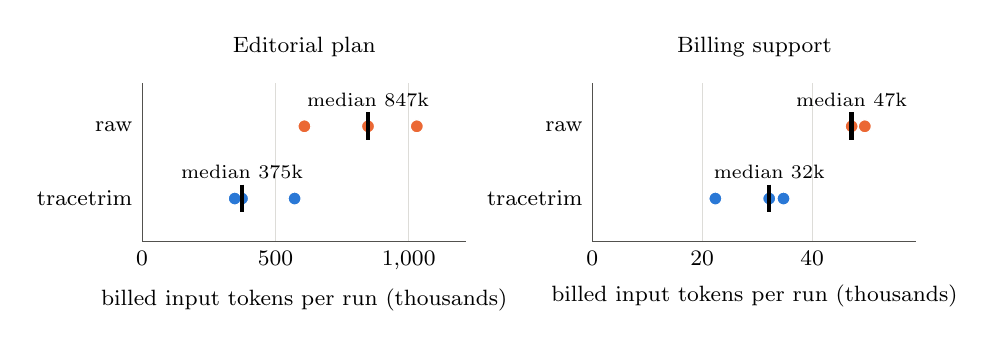
\begin{tikzpicture}
\begin{axis}[axis x line*=bottom, axis y line*=left, axis line style={draw=ttmuted}, tick style={draw=none}, major grid style={draw=ttgrid}, tick label style={font=\footnotesize}, label style={font=\footnotesize}, legend style={font=\footnotesize, draw=none, fill=none}, legend cell align=left, name=P0, width=0.47\linewidth, height=3.6cm, xmin=0, xmax=1216, xmajorgrids, symbolic y coords={tracetrim,raw}, ytick={tracetrim,raw}, enlarge y limits=0.6, xlabel={billed input tokens per run (thousands)}, title={\footnotesize Editorial plan}]
\addplot[only marks, mark=*, mark size=2.4pt, draw=white, line width=0.5pt, fill=ttorange] coordinates {(1030.4,raw) (608.7,raw) (847.3,raw)};
\addplot[mark=|, mark size=5pt, line width=1.6pt, draw=black] coordinates {(847.3,raw)} node[above=3pt, font=\scriptsize] {median 847k};
\addplot[only marks, mark=*, mark size=2.4pt, draw=white, line width=0.5pt, fill=ttblue] coordinates {(571.9,tracetrim) (374.7,tracetrim) (347.4,tracetrim)};
\addplot[mark=|, mark size=5pt, line width=1.6pt, draw=black] coordinates {(374.7,tracetrim)} node[above=3pt, font=\scriptsize] {median 375k};
\end{axis}
\begin{axis}[axis x line*=bottom, axis y line*=left, axis line style={draw=ttmuted}, tick style={draw=none}, major grid style={draw=ttgrid}, tick label style={font=\footnotesize}, label style={font=\footnotesize}, legend style={font=\footnotesize, draw=none, fill=none}, legend cell align=left, name=P1, width=0.47\linewidth, height=3.6cm, xmin=0, xmax=59, xmajorgrids, symbolic y coords={tracetrim,raw}, ytick={tracetrim,raw}, enlarge y limits=0.6, xlabel={billed input tokens per run (thousands)}, title={\footnotesize Billing support}, at={(P0.east)}, anchor=west, xshift=1.6cm]
\addplot[only marks, mark=*, mark size=2.4pt, draw=white, line width=0.5pt, fill=ttorange] coordinates {(49.6,raw) (47.2,raw) (47.2,raw)};
\addplot[mark=|, mark size=5pt, line width=1.6pt, draw=black] coordinates {(47.2,raw)} node[above=3pt, font=\scriptsize] {median 47k};
\addplot[only marks, mark=*, mark size=2.4pt, draw=white, line width=0.5pt, fill=ttblue] coordinates {(22.4,tracetrim) (32.2,tracetrim) (34.8,tracetrim)};
\addplot[mark=|, mark size=5pt, line width=1.6pt, draw=black] coordinates {(32.2,tracetrim)} node[above=3pt, font=\scriptsize] {median 32k};
\end{axis}
\end{tikzpicture}

\caption{Phase C, every run: billed input tokens per run with raw tools (orange) and with the prudent projection
and \texttt{expand} (blue); the bar marks the median. Three runs per arm: the spread is part of the result.}
\label{fig:live}
\end{figure}
